\documentclass[11pt,letter]{article}

\usepackage[]{geometry}
\geometry{
  top=1in,            % <-- you want to adjust this
  inner=1in,
  outer=1in,
  bottom=1in,
  headheight=3ex,       % <-- and this
  headsep=2ex,          % <-- and this
}
\usepackage[T1]{fontenc}
\usepackage{mathtools}
\usepackage{pifont}
\usepackage{algorithmic}
\usepackage{multirow}
\usepackage{fancyhdr}
\usepackage{amssymb}
\usepackage{multicol}
\usepackage{parskip}
\usepackage{titling}
\pretitle{\begin{flushleft}\LARGE\sffamily}
\posttitle{\par\end{flushleft}\vskip 0.5em}
\preauthor{\begin{flushleft}}
\postauthor{\par\end{flushleft}}
\predate{\begin{flushleft}\scshape}
\postdate{\par\end{flushleft}}
\setlength{\droptitle}{-20pt}
\setlength{\headheight}{15.2pt}
\pagestyle{fancy}

\providecommand{\e}[1]{\ensuremath{\times 10^{#1}}}

\fancyhf{}
\setlength{\headheight}{5pt}
\setlength\headsep{25pt}
%\renewcommand{\headrulewidth}{0pt} % remove line at top
\lhead{\fancyplain{}{CS 4780 Final Project}}
\rhead{\fancyplain{}{jc882, yl477, jp624}}
% \rfoot{\fancyplain{}{\thepage}}
\cfoot{\thepage\ of \pageref{LastPage}}
\usepackage{lastpage}

%==Bookmarks==
\usepackage{hyperref}
\hypersetup{
    % Document Information
    pdftitle={},
    pdfauthor={},
    pdfkeywords={},
    % Link Options
    colorlinks={false},
    linkcolor={white},
    pagecolor={white},
    % Display Options
    bookmarks={true},
    bookmarksopen={true},
    pdfstartview={FitH},
    pdfpagelayout={OneColumn},
    pdfpagemode={UseOutlines}}

\begin{document}
%-------------------------------------------------------------------------------
\begin{center}
% ==================TITLE PAGE==================
% Location Information
    {\large \sc Cornell University $\bullet$ Ithaca, NY}
    \vspace{42mm}
    % Title
    \\ {\huge \textbf {CS 4780 Final Project Report\vspace{8mm}\Huge\\Predicting Criminal Sentences}}
    \vspace{22mm}
    \normalsize
    % Author
    \\ Justin Cheng
    \\ Yunchi Luo
    \\ Jane\,\,\,Jae Won\,\,\,\,Park
    % Email
    \\ \{jc882, yl477, jp624\}@cornell.edu
    
    \vspace{8mm}
    
    \vspace{12mm}
    % Date
    
    December 16, 2011
 \footnote{This version was last updated and generated on \today.}
\end{center}

\vspace{20mm}

%-------------------------------------------------------------------------------
\newpage
\tableofcontents
\newpage

%-------------------------------------------------------------------------------

%\title{CS 4780 Final Project: Predicting Crimial Sentences}
%\author{Justin Cheng \emph{jc882}, Yunchi Luo \emph{yl477}, Jane Jae Won Park \emph{jp624}}
%\date{\today}
%\maketitle

%\hrule
%\vskip 1em

\section{Introduction}
\begin{quote}
``I \ldots solemnly swear that I will administer justice without respect to persons, and do equal right to the poor and to the rich, and that I will faithfully and impartially discharge and perform all the duties incumbent upon me\ldots under the Constitution and laws of the United States. So help me God.''
-- Oath of United States Justices and Judges
\end{quote}
Civilizations have adopted systems of judicial guidelines to support judges and juries in decision-making. We entrust the decision-makers to be objective and fair in their assessments of crimes without regard to factors about the offender or offense irrelevant to the offense, such as the offender's race. Yet, historically this has not always been the case--in the United States, the era of slavery and later, Jim Crow segregation lends many examples--and in many countries today someone's race or gender can be the determining factor between life and death. 

If two different individuals of different demographic backgrounds commit an identical or similar crime, will they receive the same sentence? In the U.S., the decision, after all, is made by humans who use some combination of objective sentencing criteria and subjective judgement, perhaps even whimsical impulse or personal bias. If the decisions are indeed made completely or mostly objectively, can we replace the humans with a machine instead? Countries like the Netherlands and Australia use forms of computerized sentencing to make this process more consistent and fair (Duker and Lodder). A prototype knowledge-based sentencing decision support system has been developed as well (Uri). 

While sociologists, behavioral economists, and researchers of law and our justice system have investigated how race, age and various extralegal factors affect criminal sentences, they have focused on the psychology and motivations behind these results, not the objective details of the observations themselves.  Case and offender characteristics have been found to have influence over sentence lengths (Chester). Data supports that the disposition of a trial is a heavy factor in the criminal's sentence (Ulmer). Existing studies on criminal justice, however, use traditional statistical techniques and limited case studies. Using the Pennsylvania Sentencing Data from 1998 (the most recent year available), we create several machines using combinations of machine learning techniques and different variable sets to create a machine that can determine criminal sentences and to provide an objective analysis regarding which factors of a criminal or the crime are most influential in determining the felon's sentence.

\section{Problem Definition and Methods}
Can we recover the rules judges use to determine sentences by investigating information about the criminals and sentences they received? If the judges are making purely objective decisions, is it possible to reverse-engineer parts of the law by looking at the sentences that criminals received? Can we create a machine that can, with reasonable accuracy, match the decisions of the human judges and reveal the true factors that influence sentences?
We selected input and output variables from the dataset and divided them into categories. The input variables were divided into a few sets, and combinations of these were used by machines to learn the output variables. We attempt several different learning algorithms which are detailed in following sections. These machines learn to make decisions objectively with the sole goal to become as accurate as possible in predicting the criminal's sentence. Features chosen by the machines to be the most heavily weighted in the decisions shed light into the human decision making processes. 

\subsection{Features}
We included most of the available features, filtering out ones that were redundant (e.g., a concatenation of several other fields). The variable names and descriptions are provided below
\footnote{All variables shown with postfix \_X in the form FOO\_X are actually two features, FOO\_A and FOO\_C. FOO\_A is the number of prior adjudications and FOO\_C is the number of prior convictions.}:
\begin{description}
    \item [AG\_X] Aggravated Assault (Att. SBI)
    \item [AGASBI\_X] Aggravated Assault (SBI)
    \item [AGIND\_X] Aggravated Indecent Assault
    \item [ARS\_X] Arson (F-1/No Person)
    \item [ARSPERS\_X] Arson
    \item [BUR\_X] Burglary (House and Person)
    \item [BUROTHR\_X] Burglary (other F-1)
	\item [COMPLETE] Offense Completed/Inchoate
	\item [COUNTY] Sentencing County
	\item [DAASS] Drug and Alcohol Assessment
	\item [DISP] Type of Disposition
	\item [DOB] Date of Birth
	\item [DOF] Date of Offense
	\item [DOSAGE] Age at Sentencing
	\item [DOS] Date of Sentence
	\item [DRG\_X] Other Felony Drug
	\item [DRUG50G\_X] Felony Drugs ($\ge 50g$)
	\item [DRUGDEP] Was the offender drug dependent?
	\item [DRUGDTH\_X] Drug Delivery Causing Death
	\item [ETHF1\_X] Ethnic Intimidation
	\item [F1\_X] Felony I
	\item [F2\_X] Felony II
	\item [F3\_X] Felony III
	\item [FINE] Amount of Fine Imposed
	\item [GRADE] Statutory Offense Grade
	\item [INCHOAT\_X] Inchoat to 4 pt. Offense
	\item [INCMIN] Minimum Length of Incarceration
	\item [INCMAX] Maximum Length of Incarceration
	\item [INCTYPE] Type of Incarceration
	\item [IVD\_X] Involuntary Deviate Sexual Intercourse
	\item [KID\_X] Kidnap
	\item [M1CHILD\_X] M-1 Involving Child
	\item [M1DEATH\_X] M-1 Involving Death
	\item [M1DUI\_X] M-1 DUI
	\item [MIS] Other Misdemeanor Convictions
	\item [MUR\_X] Murder
	\item [OGS] Offense Gravity Score
	\item [PCSOFF] PCS Offense Code
	\item [PCSSUB] PCS Offense Subcode
	\item [PRS] Prior Record Store
	\item [OGS] Offense Gravity Score
	\item [RACE] Ethnicity of Offender
	\item [RAP\_X] Rape
	\item [ROB\_X] Robbery (Other F-1)
	\item [ROBMV\_X] Robbery of Motor Vehicle (No SBI)
	\item [ROBSBI\_X] Robbery with SBI
	\item [ROBMVSB\_] Robbery / Motor Vehicle (SBI) 
	\item [SEX] Gender of Offender
	\item [SEXASLT\_X] Sexual Assault
	\item [SEXPRED] Is the offender a sexually violent predator?
	\item [VM\_X] Voluntary Manslaughter
	\item [WE\_X] M-1 Involving Weapon
	\item [SEX] Gender of Offender
	\item [SEXPRED] Sexually Violent Predator
\end{description}

\subsection{Datasets}

\begin{description}
	\item [DEMO] \hfill \\SEX, DOFAGE, RACE (should add DAASS in the future)
	\item [CRIME] \hfill \\FINE, GRADE, COMPLETE, DOS\_UNO, COUNTY, PCSOFF, PCSSUB, DOF\_UNO, DISP
	\item [HIST] \hfill \\MUR\_X, VM\_X, RAP\_X, KID\_X, IVD\_X, ARSPERS\_X, ROBSBI\_X, ROBMVSB\_X, AGASBI\_X, DRUGDTH\_X, BUR\_X, ETHF1\_X, INCHOAT\_X, ARS\_X, ROB\_X, ROBMV\_X, AG\_X, BUROTHR\_X, AGIND\_X, SEXASLT\_X, F1\_X, F2\_X, DRUG50G\_X, DRG\_X, F3\_X, M1DEATH\_X, WE\_X, M1CHILD\_X, M1DUI, MIS, PRS
	\item [ABOUT] \hfill \\DRUGDEP, SEXPRED
	\item [BASE] \hfill \\Features from both DEMO and CRIME
	\item [ALL] \hfill \\Features from DEMO, CRIME, HIST and ABOUT
\end{description}
The DEMO subset only contains demographic information, while the CRIME subset contains only details about the offense committed. HIST contains variables about the offender's prior offense records, and ABOUT contains two descriptions of the offender.

\subsection{Feature Processing}
\begin{description}
	\item [\emph{b/nb} Binarization] 'Split' a multi-valued label into multiple binary variables for each label (i.e., one-hot encoding of the label)
	\item [\emph{c/nc} Coarsification] Place continuous data into a number of evenly distributed buckets, so that there are fewer values to work with.
	\item [\emph{\_/uno} Date field separation] Process date data (MM/DD/YYYY) into month, day, year, day of week, or unix time.
	\item [\emph{\_/balN}] Sorting label values into $N$ buckets, and whether the sample contained equal number of examples from each bucket
\end{description}


\subsection{Variable Correlation}
We performed linear regression on all pairs of attributes, and calculated the correlation coefficient, $\rho_{X,Y} = \frac{cov(X,Y)}{\sigma_X\sigma_Y}$, for each of them. To validate the correlation coefficients obtained, we calculated the $p$-value for the null hypothesis that the correlation coefficient of two attributes is 0.

\subsection{Learning Algorithms}
We used C4.5 decision trees, linear SVM, logistic regression, naive bayes, k-nearest neighbors, and SVM with kernels (via SVMLight).

\subsubsection{Decision Tree Learning}

We used an the Orange implementation of the C4.5 Decision Tree Algorithm.

\paragraph{Parameter Tuning}
Parameter tuning was carried out by trying out all possible combinations of parameters below, using the classification accuracy obtained on 10-fold cross-validation.

\begin{itemize}
	\item Parameter $m$ from $0.1$ to $100$ \\
		- Parameter used in computing M-estimate probabilities during post-pruning
	\item Maximum majority from $0.5$ to $1.0$ \\
		- Induction stops when a node has a majority at least this value
	\item Minimum examples per node from $0$ to $10$ \\
		- Minimum examples in each leaf
	\item Minimum subset from $0$ to $10$ \\
		- Minimum examples in non-null leaves
	\item Measures - information gain, information gain ratio, gini index, relief % See http://orange.biolab.si/doc//orange25/Orange.feature.scoring.html#Orange.feature.scoring.Relief
\end{itemize}

\subsubsection{kNN Learning}

\paragraph{Parameter Tuning}
\begin{itemize}
	\item $k$ from $1$ to $2\sqrt{n}$ \\
		- Since a good value of $k$ to use is generally $\sqrt{n}$
\end{itemize}

\subsection{Regression}
In addition to the binary classification task detailed above, we also used regression to find out how well we could predict features like INCMIN if they were instead continuous. We used two methods - linear regression, and SVM regression. The reason for the use of these two methods is that linear regression is fast and in many cases a sufficient model in regression classification tasks. SVM regression, while significantly slower, allows the use of kernels which could possibly improve our accuracy, which we quantify in terms of the Akaike information criterion (AIC) and $R^2$.

We also employ the use of principle component analysis (PCA), in order to better understand which features can best predict our target variable, as well as explore the possibility of reducing the dimensionality of our data without sacrificing accuracy (i.e. principle component regression, or using the components generated by PCA in linear regression).

As in the binary task, we trained a regression classifier on 80\% of the data, while validating it on the remaining 20\%.

\section{Experimental Evaluation}
\subsection{Methdology}
TODO: overview of evaluation methodology, what we used to measure performance

TODO: training/test data used, why is it realistic or interesting?

\subsection{Results}
TODO: change all tables to charts
\subsubsection{Cross-Validation Set Accuracy}
The classification accuracies listed below is the accuracy obtained on 10-fold cross-validation.

CA is the classification accuracy, TP is the number of true positives, FP is the number of false positives, FN is the number of false negatives, TN is the number of true negatives.

\textbf{DEMO} \\
\begin{tabular}{|l|c|c|c|c|c|c|c|}
\hline
Algorithm & CA & TP & FP & FN & TN & Precision & Recall\\
\hline
c4.5   	 & 0.905 & 5554  & 423  &  794   & 5982 & 0.929 & 0.875\\
linsvm 	 & 0.882 & 4996  & 150  &  1352  & 6255 & 0.971 & 0.787\\
logreg 	 & 0.882 & 4991  & 149  &  1357  & 6256 & 0.971 & 0.786\\
bayes  	 & 0.861 & 5274  & 694  &  1074  & 5711 & 0.884 & 0.831\\
knn   & 0.905 & 5667  & 535  &  681   & 5870 & 0.914 & 0.893\\
svmlight & 0.889 & 5046  & 167	&  1302	 & 6238 & 0.968 & 0.795\\ 
\hline
\end{tabular}

\textbf{CRIME} \\
\begin{tabular}{|l|c|c|c|c|c|c|c|}
\hline
Algorithm & CA & TP & FP & FN & TN & Precision & Recall\\
\hline
c4.5     & 0.821  &  4484  &  1003  &  926   &  4348 & 0.817 & 0.829\\
linsvm   & 0.819  &  4605  &  1147  &  805   &  4204 & 0.801 & 0.851\\
logreg   & 0.819  &  4613  &  1152  &  797   &  4199 & 0.800 & 0.853\\
bayes    & 0.810  &  4394  &  1029  &  1016  &  4322 & 0.810 & 0.812\\
knn   & 0.822  &  4485  &  995   &  925   &  4356 & 0.818 & 0.829\\
svmlight & 0.831  &  4632  &  1077  &  778   &  4274 & 0.811 & 0.856\\
\hline
\end{tabular}

\textbf{BASE} \\
\begin{tabular}{|l|c|c|c|c|c|c|c|}
\hline
Algorithm & CA & TP & FP & FN & TN & Precision & Recall\\
\hline
c4.5     & 0.923 & 4823 & 356  &  458   &  4947 & 0.931 & 0.913\\ 
linsvm   & 0.919 & 4716 & 293  &  565   &  5010 & 0.942 & 0.893\\ 
logreg   & 0.919 & 4710 & 291  &  571   &  5012 & 0.942 & 0.892\\ 
bayes    & 0.886 & 4897 & 820  &  384   &  4483 & 0.857 & 0.927\\
knn   & 0.896 & 4647 & 464  &  634   &  4839 & 0.909 & 0.880\\
svmlight & 0.925 & 4822 & 313  &  459   &  4990 & 0.939 & 0.913\\
\hline
\end{tabular}

\textbf{CRIME + HISTORY} \\
\begin{tabular}{|l|c|c|c|c|c|c|c|}
\hline
Algorithm & CA & TP & FP & FN & TN & Precision & Recall\\
\hline
c4.5     & 0.817 & 4344  & 953   & 1012 &  4452 & 0.820 & 0.811\\ 
linsvm   & 0.811 & 4447  & 1121  & 909  &  4284 & 0.799 & 0.830\\
logreg   & 0.812 & 4475  & 1140  & 881  &  4265 & 0.797 & 0.836\\ 
bayes    & 0.807 & 4311  & 1029  & 1045 &  4376 & 0.807 & 0.805\\ 
knn   & 0.817 & 4375  & 986   & 981  &  4419 & 0.816 & 0.817\\ 
svmlight & 0.823 & 4541  & 1103  & 815  &  4302 & 0.805 & 0.848\\
\hline
\end{tabular}

\begin{figure}
	\centering
	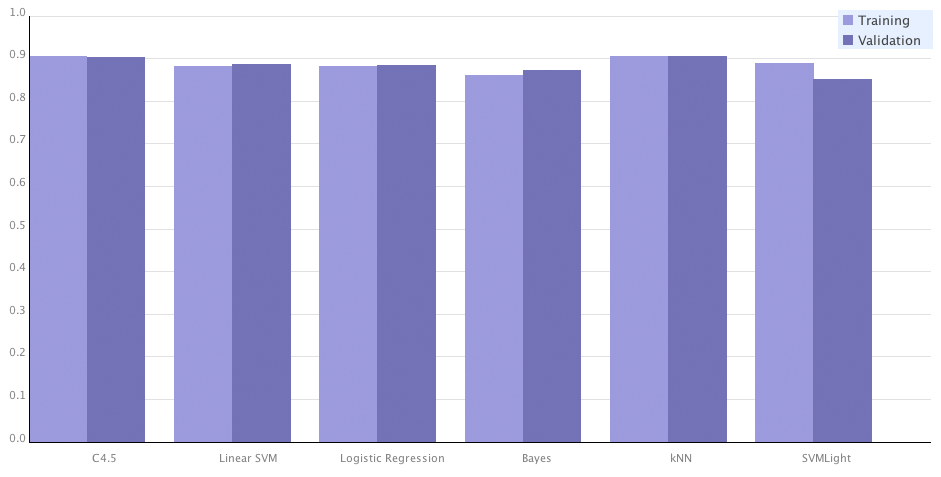
\includegraphics[scale=0.4]{report_figures/tv_accuracy_bar.png}
	\caption{Training set vs validation set accuracy for DEMO}
\end{figure}

\subsubsection{Validation Set Accuracy}

\begin{figure}
	\centering
	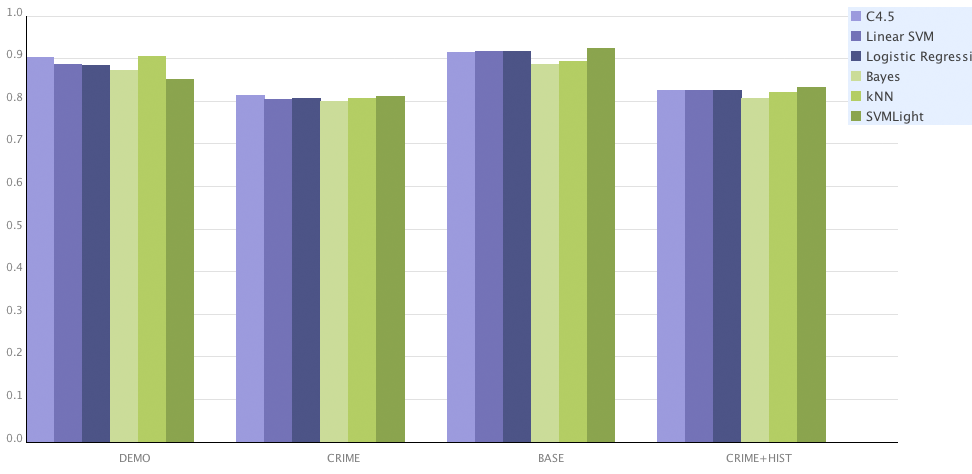
\includegraphics[scale=0.4]{report_figures/val_accuracy_bar.png}
	\caption{Validation set accuracy}
\end{figure}

\begin{tabular}{|l|c|c|c|c|c|}
\hline
Algorithm & DEMO & CRIME & BASE & CRIME + HISTORY\\
\hline
c4.5     & 0.903 & 0.814 & 0.915 & 0.826 \\
linsvm   & 0.885 & 0.804 & 0.916 & 0.826 \\
logreg   & 0.884 & 0.806 & 0.916 & 0.824 \\
bayes    & 0.871 & 0.799 & 0.886 & 0.807 \\
knn   & 0.905 & 0.806 & 0.893 & 0.821 \\
svmlight & 0.852 & 0.811 & 0.924 & 0.832 \\
\hline
\end{tabular}

\subsubsection{Validation Set Precision}

\begin{tabular}{|l|c|c|c|c|c|}
\hline
Algorithm & DEMO & CRIME & BASE & CRIME + HISTORY\\
\hline
c4.5     & 0.928 & 0.810 & 0.924 & 0.834 \\
linsvm   & 0.976 & 0.784 & 0.936 & 0.810 \\
logreg   & 0.976 & 0.782 & 0.934 & 0.810 \\
knn   & 0.915 & 0.806 & 0.908 & 0.823 \\
bayes    & 0.895 & 0.796 & 0.854 & 0.813 \\
svmlight & 0.825 & 0.793 & 0.931 & 0.821 \\
\hline
\end{tabular}

\subsubsection{Validation Set Recall}

\begin{tabular}{|l|c|c|c|c|c|}
\hline
Algorithm & DEMO & CRIME & BASE & CRIME + HISTORY\\
\hline
c4.5     & 0.878 & 0.809 & 0.907 & 0.821 \\
linsvm   & 0.794 & 0.827 & 0.896 & 0.859 \\
logreg   & 0.791 & 0.828 & 0.898 & 0.855 \\
knn   & 0.847 & 0.796 & 0.876 & 0.825 \\
bayes    & 0.896 & 0.793 & 0.933 & 0.807 \\
svmlight & 0.900 & 0.831 & 0.918 & 0.855 \\
\hline
\end{tabular}

\subsubsection{Variable Correlation}

\textbf{Correlation Heat Map}
\begin{figure}
	\centering
	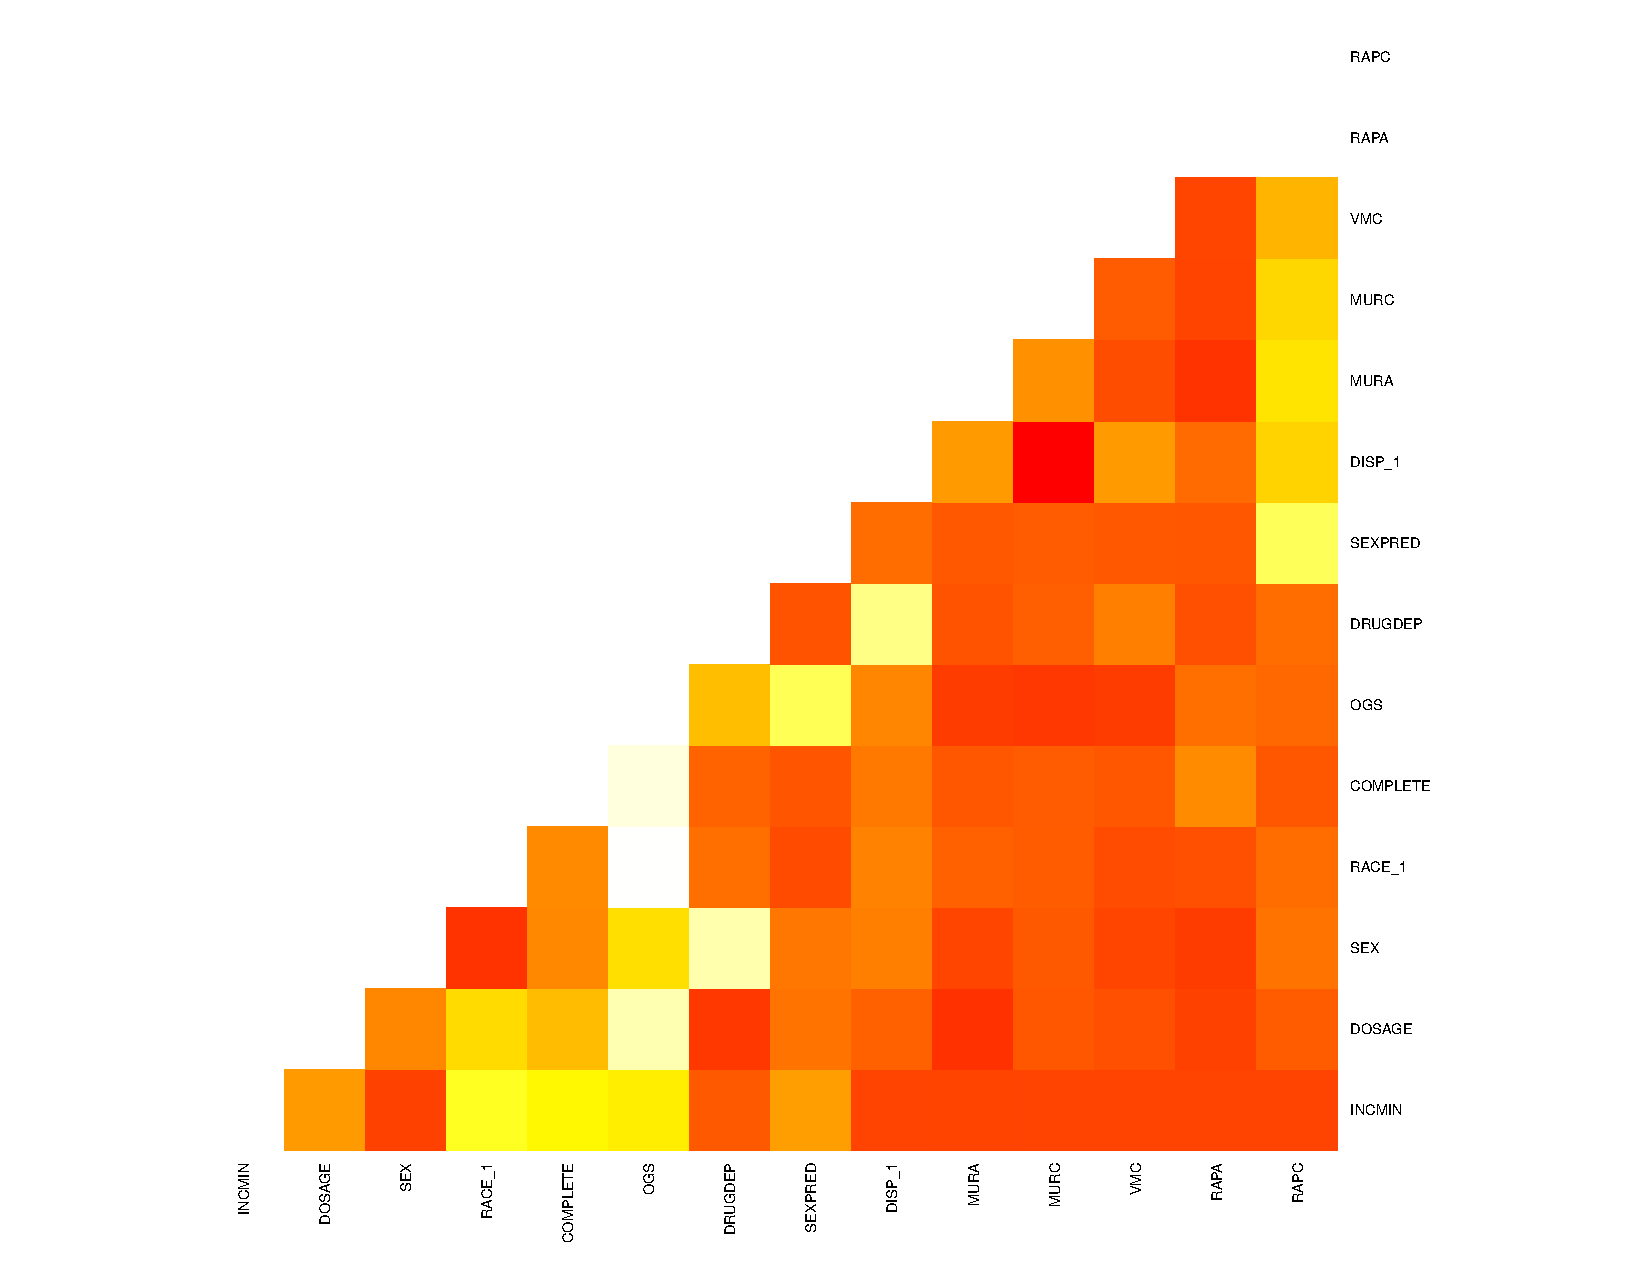
\includegraphics[scale=0.35]{report_figures/cool.pdf}
	\caption{Correlation heat map for selected features}
	\label{corr_heat_map}
\end{figure}
Figure \ref{corr_heat_map} shows the strength of correlation between selected attributes. For instance, there is a high correlation between $RACE\_1$ and $INCMIN$, suggesting that whites receive shorter sentences overall. In addition, looking at $OGS$ and $RACE\_1$, whites have lower offense gravity scores (OGS) on average. Additionally, if someone completed a crime (COMPLETE), it was more likely that that that person got a longer minimum sentence (INCMIN).

The correlation heat maps in the appendix show the correlation between all tested attributes.

\textbf{Top Correlated Attributes}
Ignoring correlation between binarized attributes (ex. GRADE\_1 and GRADE\_2), 
and trivial correlations such as that between DOSAGE and DOFAGE and PCSOFF and GRADE (since unique PCSOFFs are assigned unique GRADEs in the codebook), we obtain

\begin{tabular}{|l|l|r|c|}
\hline
Attribute $X$ & Attribute $Y$ & $\rho_{X,Y}$ & $p$-value \\
\hline
COUNTY\_1 & PCSOFF\_182902 & 0.817 & 2.2\e{-16} \\
PCSOFF\_183301 & ARSA & 0.628 & 2.2\e{-16} \\
COUNTY\_53 & PCSOFF\_184905 & 0.577 & 2.2\e{-16} \\
PCSOFF\_757122 & M1DUIC & 0.576 & 2.2\e{-16} \\
ROBA & WEA & 0.547 & 2.2\e{-16} \\
COUNTY\_51 & DISP\_4 & 0.541 & 2.2\e{-16} \\
F1A & ROBSBIC & 0.534 & 2.2\e{-16} \\
MIS & PRS & 0.513 & 2.2\e{-16} \\
PCSOFF\_185506 & SEXASLTC & 0.500 & 2.2\e{-16} \\
COUNTY\_39 & PCSOFF\_183301 & 0.490 & 2.2\e{-16} \\
%COUNTY\_37&	DISP\_6&	0.69581896 & 2.2e-16\\
%INCMIN&	GRADE&	0.51992742 & 2.2e-16\\
%COUNTY\_47&	PCSOFF\_180912&	0.44711808 & 2.2e-16\\
%INCMIN&	PCSOFF\_753731&	0.44359416 & 2.2e-16\\
%COUNTY\_51&	DISP\_4&	0.40880622 & 2.2e-16\\
%RACE\_1&	COUNTY\_51&	0.38671562 & 2.2e-16\\
%INCMIN&	PCSSUB\_A&	0.34272914 & 2.2e-16\\
%RACE\_2&	COUNTY\_51&	0.33313766 & 2.2e-16\\
%RACE\_1&	PCSOFF\_753731&	0.3129321 & 2.2e-16\\
%COUNTY\_9&	DISP\_2&	0.31041962 & 2.2e-16\\
\hline
\end{tabular}

For example, according to the high correlation between $COUNTY\_1$ and $PCSOFF\_182902$, if you're convicted in Adams county, you're likely to have unlawfully restrained someone and vice versa. If you've had prior arson adjudications, you've probably committed arson again. Somewhat unexpectedly, if you've had prior DUI convictions, you've probably altered or forged vehicle license plates. If you've had a prior robbery adjudication, naturally you've also probably had a weapon misdemeanor adjudication.

\subsubsection{Decision Tree}
\textbf{Optimal Parameters}

\begin{tabular}{|c|c|c|c|c|c|c|}
\hline
Dataset & $m$ & Max. majority & Min. examples & Min. subset & Measure & Accuracy \\
\hline
DEMO & 5 & 1.0 & 2 & 2 & Gini & 0.659 \\
CRIME & 100 & 1.0 & 2 & 2 & Relief & 0.783 \\
BASE & 100 & 0.8 & 1 & 2 & Relief & 0.774 \\
\hline
\end{tabular}

\paragraph{Optimal Decision Tree for DEMO} % TODO Turn this into a pretty tree?
\begin{verbatim}
RACE_1=0
|    SEX=1
|    |    DOFAGE<=39.500: 1 (69.05%)
|    |    DOFAGE>39.500
|    |    |    RACE_9=1: -1 (100.00%)
|    |    |    RACE_9=0
|    |    |    |    . . .
|    SEX=2
|    |    RACE_9=1: -1 (100.00%)
|    |    RACE_9=0
|    |    |    DOFAGE<=32.000: 1 (61.54%)
|    |    |    DOFAGE>32.000
|    |    |    |    . . .
RACE_1=1
|    DOFAGE<=24.500
|    |    DOFAGE<=19.500
|    |    |    DOFAGE<=17.500: 1 (80.00%)
|    |    |    DOFAGE>17.500: -1 (75.47%)
|    |    DOFAGE>19.500
|    |    |    SEX=1: 1 (57.94%)
|    |    |    SEX=2: -1 (83.33%)
|    DOFAGE>24.500
|    |    DOFAGE<=38.500: -1 (70.00%)
|    |    DOFAGE>38.500
|    |    |    DOFAGE>43.500: -1 (76.92%)
|    |    |    DOFAGE<=43.500
|    |    |    |    . . .
\end{verbatim}

\subsubsection{SVM}
\begin{tabular}{|c|c|c|c|c|}
\hline
Dataset & $C$ & $t$ & $t$-dependent. vars & Accuracy \\
\hline
DEMO & 5 & 2 (RBF) & $g=0.05$ & 0.651 \\
\hline
\end{tabular}

\subsubsection{kNN}
\begin{tabular}{|c|c|c|}
\hline
Dataset & $k$ & Accuracy \\
\hline
DEMO & 55 & 0.643 \\
CRIME & 28 & 0.769 \\
BASE & 42 & 0.773 \\
\hline
\end{tabular}


\subsubsection{Significance Tests}

\textbf{Binomial Sign Test}
The binomial sign test was used to evaluate whether an algorithm performed better ($p=0.05$) than another for each dataset. Each cell in the table below corresponds to whether the learning algorithm in that row was significantly BETTER than the algorithm in that column, WORSE or similar ($\sim$).

\textbf{Note:} C4.5, Linear SVM, kNN, and SVMLight are all tuned using 10-fold cross-validation.

\paragraph{DEMO} \quad

\begin{tabular}{|c|c|c|c|c|c|c|}
\hline
Algorithm & C4.5  & Linear SVM & Log. Reg.  & kNN  & Bayes & SVMLight \\
\hline
C4.5 	& -		& BETTER	& BETTER	& $\sim$	& BETTER	& BETTER	\\
Linear SVM		& -		& -			& $\sim$	& WORSE		& BETTER	& BETTER	\\
Log. Reg. 	& -		& -			& -			& WORSE		& BETTER	& BETTER	\\
kNN 		& -		& -			& -			& -			& BETTER	& BETTER	\\
Bayes			& -		& -			& -			& -			& -			& BETTER	\\
SVMLight & - & - & - & - & - & - \\
\hline
\end{tabular}

\paragraph{CRIME} \quad

\begin{tabular}{|c|c|c|c|c|c|c|}
\hline
Algorithm & C4.5  & Linear SVM & Log. Reg. & kNN  & Bayes & SVMLight \\
\hline
C4.5 	& -		& $\sim$	& $\sim$	& $\sim$	& BETTER	& $\sim$	\\
Linear SVM		& -		& -			& $\sim$	& $\sim$	& $\sim$	& $\sim$	\\
Log. Reg. 	& -		& -			& -			& $\sim$	& $\sim$	& WORSE 	\\
kNN 		& -		& -			& -			& -			& $\sim$	& $\sim$	\\
Bayes			& -		& -			& -			& -			& -			& WORSE		\\
SVMLight & - & - & - & - & - & - \\
\hline
\end{tabular}

\paragraph{BASE} \quad

\begin{tabular}{|c|c|c|c|c|c|c|}
\hline
Algorithm & C4.5  & Linear SVM & Log. Reg.  & kNN  & Bayes & SVMLight \\
\hline
C4.5 	& -		& $\sim$	& $\sim$	& BETTER	& BETTER	& WORSE		\\
Linear SVM		& -		& -			& $\sim$	& BETTER	& BETTER	& WORSE		\\
Log. Reg. 	& -		& -			& -			& BETTER	& BETTER	& WORSE 	\\
kNN 		& -		& -			& -			& -			& $\sim$	& WORSE		\\
Bayes			& -		& -			& -			& -			& -			& WORSE		\\
SVMLight & - & - & - & - & - & - \\
\hline
\end{tabular}

\paragraph{CRIME + HISTORY} \quad

\begin{tabular}{|c|c|c|c|c|c|c|}
\hline
Algorithm & C4.5  & Linear SVM & Log. Reg.  & kNN  & Bayes & SVMLight \\
\hline
C4.5 	& -		& $\sim$	& $\sim$	& $\sim$	& BETTER	& $\sim$		\\
Linear SVM		& -		& -			& $\sim$	& $\sim$	& BETTER	& $\sim$		\\
Log. Reg. 	& -		& -			& -			& $\sim$	& BETTER	& $\sim$ 	\\
kNN 		& -		& -			& -			& -			& BETTER	& WORSE		\\
Bayes			& -		& -			& -			& -			& -			& WORSE		\\
SVMLight & - & - & - & - & - & - \\
\hline
\end{tabular}


\subsubsection{Regression Analysis}

\textbf{Linear Regression}
The results of linear regression on each dataset are summarized in Table \ref{TableLinReg}. Here, we see that AIC is lowest for ALL, given that every other feature set is a subset of it. Surprisingly, ABOUT, despite having only 2 features, best predicts minimum incarceration. Nevertheless, we see here that using demographic features (DEMO) results in the highest AIC score, again demonstrating that by-and-large, sentences lengths are decided independent of one's age, gender or race.

\begin{table}[h]
  \centering
  \begin{tabular}{|c|c|c|c|c|c|}
  \hline
  Dataset & AIC & $R^2$ & Attr. & Coeff. & $p$-value \\
  \hline
  \multirow{2}{*}{DEMO} & \multirow{2}{*}{9.00\e{4}} & \multirow{2}{*}{1.40\e{-2}} & COUNTY\_48 & 0.249 & 2\e{-16} \\
  &&& COUNTY\_39 & 0.183 & 4.73\e{-16} \\
  \hline
  \multirow{2}{*}{CRIME} & \multirow{2}{*}{7.41\e{4}} & \multirow{2}{*}{3.55\e{-2}} & PCSOFF\_751543 & 2.76 & 4.73\e{-7} \\
  &&& PCSOFF\_353009 & 1.34 & 1.19\e{-2} \\  
  \hline
  \multirow{2}{*}{ABOUT} & \multirow{2}{*}{1.57\e{4}} & \multirow{2}{*}{3.44\e{-3}} & SEXPRED & -3.78\e{-1} & 8.55\e{-4} \\
  &&& - & - & - \\  
  \hline
  \multirow{2}{*}{HIST} & \multirow{2}{*}{2.86\e{4}} & \multirow{2}{*}{-7.82\e{-3}} & RAPC & 7.28\e{-1} & 3.49\e{-4} \\
  &&& F1C & 7.34\e{-2} & 4.43\e{-3} \\
  \hline
  \multirow{2}{*}{ALL} & \multirow{2}{*}{4.48\e{3}} & \multirow{2}{*}{1.77\e{-3}} & PCSOFF\_185503 & 1.08 & 3.58\e{-3} \\
  &&& COMPLETE & 1.97\e{-1} & 2.68\e{-4} \\
  \hline
  \end{tabular}
  \caption{Linear regression listing components with the highest coefficients (COUNTY\_48 - Northampton; COUNTY\_39 - Lehigh; PCSOFF\_751543 - driving with a suspended license; PCSOFF\_353009 - Possession with intent to distribute; SEXPRED - Sexually violent predator; RAPC - prior rape conviction; F1C - other felony conviction; PCSOFF\_185503 - disorderly conduct; COMPLETE - offense completed)}
  \label{TableLinReg}
\end{table}

\textbf{Principle Component Regression}
Principle component decomposition was performed on each dataset, and the top components generated, by proportion of variance in the dataset explained (so that $\#=1$ refers to the component that explains the most variance), are listed in Table \ref{TablePCR1}, along with the attributes with the highest weights that make up each component. Table \ref{TablePCR2} shows the results of linear regression on the transformed components. 

In most cases, the components that have the highest coefficients in the linear regression are not the ones that explain the most variance. For example, \# 17 and 18 for DEMO correspond to the components which weigh $COUNTY\_48$ (Northampton) and $COUNTY\_54$ (Schuylkill) most.

\begin{table}[h]
  \centering
  \begin{tabular}{|c|c|c|l|}
  \hline
  Dataset & \# & V.E. & Top 5 Components \\
  \hline
  \multirow{2}{*}{DEMO} & 1 & 2.70\e{-1} & RACE1, COUNTY67, COUNTY40, COUNTY54, SEX \\
  & 2 & 7.16\e{-2} & SEX, RACE2, COUNTY2, RACE1, COUNTY23 \\
  \hline
  \multirow{2}{*}{CRIME} & 1 & 1.84\e{-1} & PCSSUB\_B, OGS, PCSSUB\_D, PCSOFF183502, PCSOFF183701 \\
  & 2 & 1.57\e{-1} & DISP2, OGS, DISP4, PCSSUB\_B, DISP5 \\
  \hline
  \multirow{2}{*}{ABOUT} & 1 & 9.67\e{-1} & DRUGDEP, SEXPRED \\
  & 2 & 3.27\e{-2} & SEXPRED, DRUGDEP \\
  \hline
  \multirow{2}{*}{HIST} & 1 & 4.13\e{-1} & PRS, MIS, F3C, DRGC, F1C \\
  & 2 & 1.29\e{-1} & MIS, AGC, M1CHILDA, WEA, M1DUIA  \\
  \hline
  \multirow{2}{*}{ALL} & 1 & 1.20\e{-1} & RACE1, PCSOFF753731, PCSSUB\_A, DISP1, DOFUNO \\
  & 2 & 8.55\e{-2} & MIS, PRS, F3C, PCSSUB\_A, DOFUNO \\
  \hline
  \end{tabular}
  \caption{PCA decomposition listing top components (\#) by variance explained (V.E.) and makeup}
  \label{TablePCR1}
\end{table}

\begin{table}[h]
  \centering
  \begin{tabular}{|c|c|c|c|c|c|c|}
  \hline
  Dataset & AIC & $R^2$ & \# & V.E. & Coeff. & $p$-value \\
  \hline
  \multirow{2}{*}{DEMO} & \multirow{2}{*}{9.00\e{4}} & \multirow{2}{*}{1.40\e{-2}} & 17 & 1.19\e{-2} & 2.05\e{-1} & <2\e{-16} \\
  &&& 18 & 1.14\e{-2} & -2.07\e{-1} & <2\e{-16} \\
  \hline
  \multirow{2}{*}{CRIME} & \multirow{2}{*}{7.41\e{4}} & \multirow{2}{*}{3.55\e{-2}} & 111 & 1.03\e{-4} & -1.64 & 2.58\e{-15} \\
  &&& 113 & 1.02\e{-4} & -1.89 & <2\e{-16} \\  
  \hline
  \multirow{2}{*}{ABOUT} & \multirow{2}{*}{1.57\e{4}} & \multirow{2}{*}{3.44\e{-3}} & 2 & 3.27\e{-2} & 1.19\e{-2} & 8.55\e{-4} \\
  &&& - & - & - & - \\  
  \hline
  \multirow{2}{*}{HIST} & \multirow{2}{*}{2.86\e{4}} & \multirow{2}{*}{-7.82\e{-3}} & 37 & 7.21\e{-4} & 5.97\e{-1} & 7.71\e{-3} \\
  &&& 30 & 1.14\e{-3} & -3.54\e{-1} & 4.67\e{-2} \\
  \hline
  \multirow{2}{*}{ALL} & \multirow{2}{*}{4.48\e{3}} & \multirow{2}{*}{1.77\e{-3}} & - & - & - & - \\
  &&& - & - & - & - \\
  \hline
  \end{tabular}
  \caption{PCR listing significant components with the highest absolute coefficients}
  \label{TablePCR2}
\end{table}

\textbf{SVM Regression}
SVM regression was also performed, and the results summarized in Table \ref{TableSVMReg}.
\begin{table}[h]
  \centering
  \begin{tabular}{|c|c|c|c|c|c|}
  \hline
  Dataset & $R^2$ & MSE & Attr. & Coeff. \\
  \hline
  \multirow{2}{*}{DEMO*} & \multirow{2}{*}{-5.40\e{-3}} & \multirow{2}{*}{9.33\e{3}} & COUNTY\_1 & 6.23\e{-2} \\
  &&& COUNTY\_51 & 3.19\e{-2} \\
  \hline
  \multirow{2}{*}{CRIME} & \multirow{2}{*}{7.94\e{-3}} & \multirow{2}{*}{6.38\e{3}} & PCSOFF\_182502 & 2.58\e{-1} \\
  &&& OGS & 1.86\e{-1} \\  
  \hline
  \multirow{2}{*}{ABOUT} & \multirow{2}{*}{-4.07\e{-3}} & \multirow{2}{*}{1.35\e{3}} & SEXPRED & -6.31\e{-2} \\
  &&& DRUGDEP & -3.61\e{-4} \\  
  \hline
  \multirow{2}{*}{HIST} & \multirow{2}{*}{-8.59\e{-3}} & \multirow{2}{*}{2.73\e{3}} & ETHF1A & 9.82\e{-2} \\
  &&& INCHOATA & 6.63\e{-2} \\
  \hline
  \end{tabular}
  \caption{SVM regression listing components with the highest coefficients (in linear case) (COUNTY\_1 - Adams; COUNTY\_51 - Philadelphia, ETHF1A - Prior ethnic intimidation adjudication; INCHOATA - Prior inchoate adjudication) (*Excluding DOSAGE)}
  \label{TableSVMReg}
\end{table}

\subsection{Discussion}
TODO

\section{Related Work}
Many studies have investigated the influence of extralegal factors in sentencing. Johnson analyzes the Pennsylvania Sentencing Data specifically on sentences that depart from guidelines. His results suggest that black and hispanic defendants compared to whites, men compared to women, and younger offenders compared to older ones are more likelier to receive a sentence that deviates in an unfavorable direction from the guidelines. Johnson also notes that combinations of variables, like race and mode of conviction, serve as strong indicators of the direction that a sentence will deviate in. 

Sentencing decision support systems have been of interest in AI, but we do not know of any such studies that have been done in machine learning. As mentioned in the introduction, some countries are moving towards delegating the gathering of information needed for sentencing to machines instead of humans. These programs do not replace judges (yet), but generally tell judges what other judges have decided for similar cases. 
The Sentencing Information System of Scotland allows judges to enter information about the offender and offense to view the decisions that other judges made for similar circumstances, to help judges to keep sentences consistent. Uri notes that ``most people\ldots believe that as a matter of \emph{principle} [the tasks of a judge] should be an exclusively human one.'' This conception is unlikely to change anytime soon, given the popular fear and mistrust of machines. 


\section{Future Work}
We did not have the time to investigate sentencing output variables other than INCMIN, the minimum incarceration time. A court sentence is a multi-dimensional output, so future work should also look at output variables like INCMAX (maximum incarceration time), INCTYPE (type of incarceration), FINE (fine charged), etc. 

Also, we binarified INCMIN to indicate only whether the sentence was greater than 12 months for all methods except for regression. Since INCMIN is originally a continous variable, future work should look at continuous outputs, or at least coarsified (rather than binarified) outputs. The same applies for the other potential output variables as well. Such studies take into account that the output variables are not independent of one another. e.g., a greater INCMIN may be associated with a lesser FINE. 

We computed variable correlation, but did not take the data into account in creating the sentence predictors. Taking the correlation into account -----.

\section{Conclusion}

\section{References}
\begin{enumerate}
\item Britt, Chester L., "Modeling the distribution of sentence length decisions under a guidelines system: An application of quantile regression models." Journal of Quantitative Criminology. Dec 2009, 25, (4), 341 - 370. DOI: 10.1007/s10940-009-9066-x
\item Johnson, Brian D., "Racial and ethnic disparities in sentencing departures across modes of conviction." Criminology. May 2003, 41, (2), 449 - 489. DOI: 10.1111/j.1745-9125.2003.tb00994.x
\item Ullmer, Jefferey T.; Johnson, Brian, "Sentencing in context: A multilevel analysis." Criminology. Feb 2004, 42, (1), 137 - 177. DOI: 10.1111/j.1745-9125.2004.tb00516.x
\item Ulmer, Jeffery T.; Bradley, Minda S., "Variation in trial penalties among serious violent offenses." Criminology. Aug 2006, 44, (3), 631 - 670. DOI: 10.1111/j.1745-9125.2006.00059.x
\item Uri J. Schild and Ruth Kannai. 2003. Intelligent computer evaluation of offender's previous record. In Proceedings of the 9th international conference on Artificial intelligence and law (ICAIL '03). ACM, New York, NY, USA, 185-194. DOI=10.1145/1047788.1047831 http://doi.acm.org/10.1145/1047788.1047831
\item Uri J. Schild. 1995. Intelligent computer systems for criminal sentencing. In Proceedings of the 5th international conference on Artificial intelligence and law (ICAIL '95). ACM, New York, NY, USA, 229-238. DOI=10.1145/222092.222247 http://doi.acm.org/10.1145/222092.222247
\item Marius J. A. Duker and Arno R. Lodder. 1999. Sentencing and information management: consistency and the particularities of a case. In Proceedings of the 7th international conference on Artificial intelligence and law (ICAIL '99). ACM, New York, NY, USA, 100-107. DOI=10.1145/323706.323720 http://doi.acm.org/10.1145/323706.323720
\end{enumerate}
\section{Appendix}

\subsection{Correlation Heat Maps}
Red indicates low correlation, light yellow indicates high correlation.
\subsubsection{DEMO Correlation Heat Map}
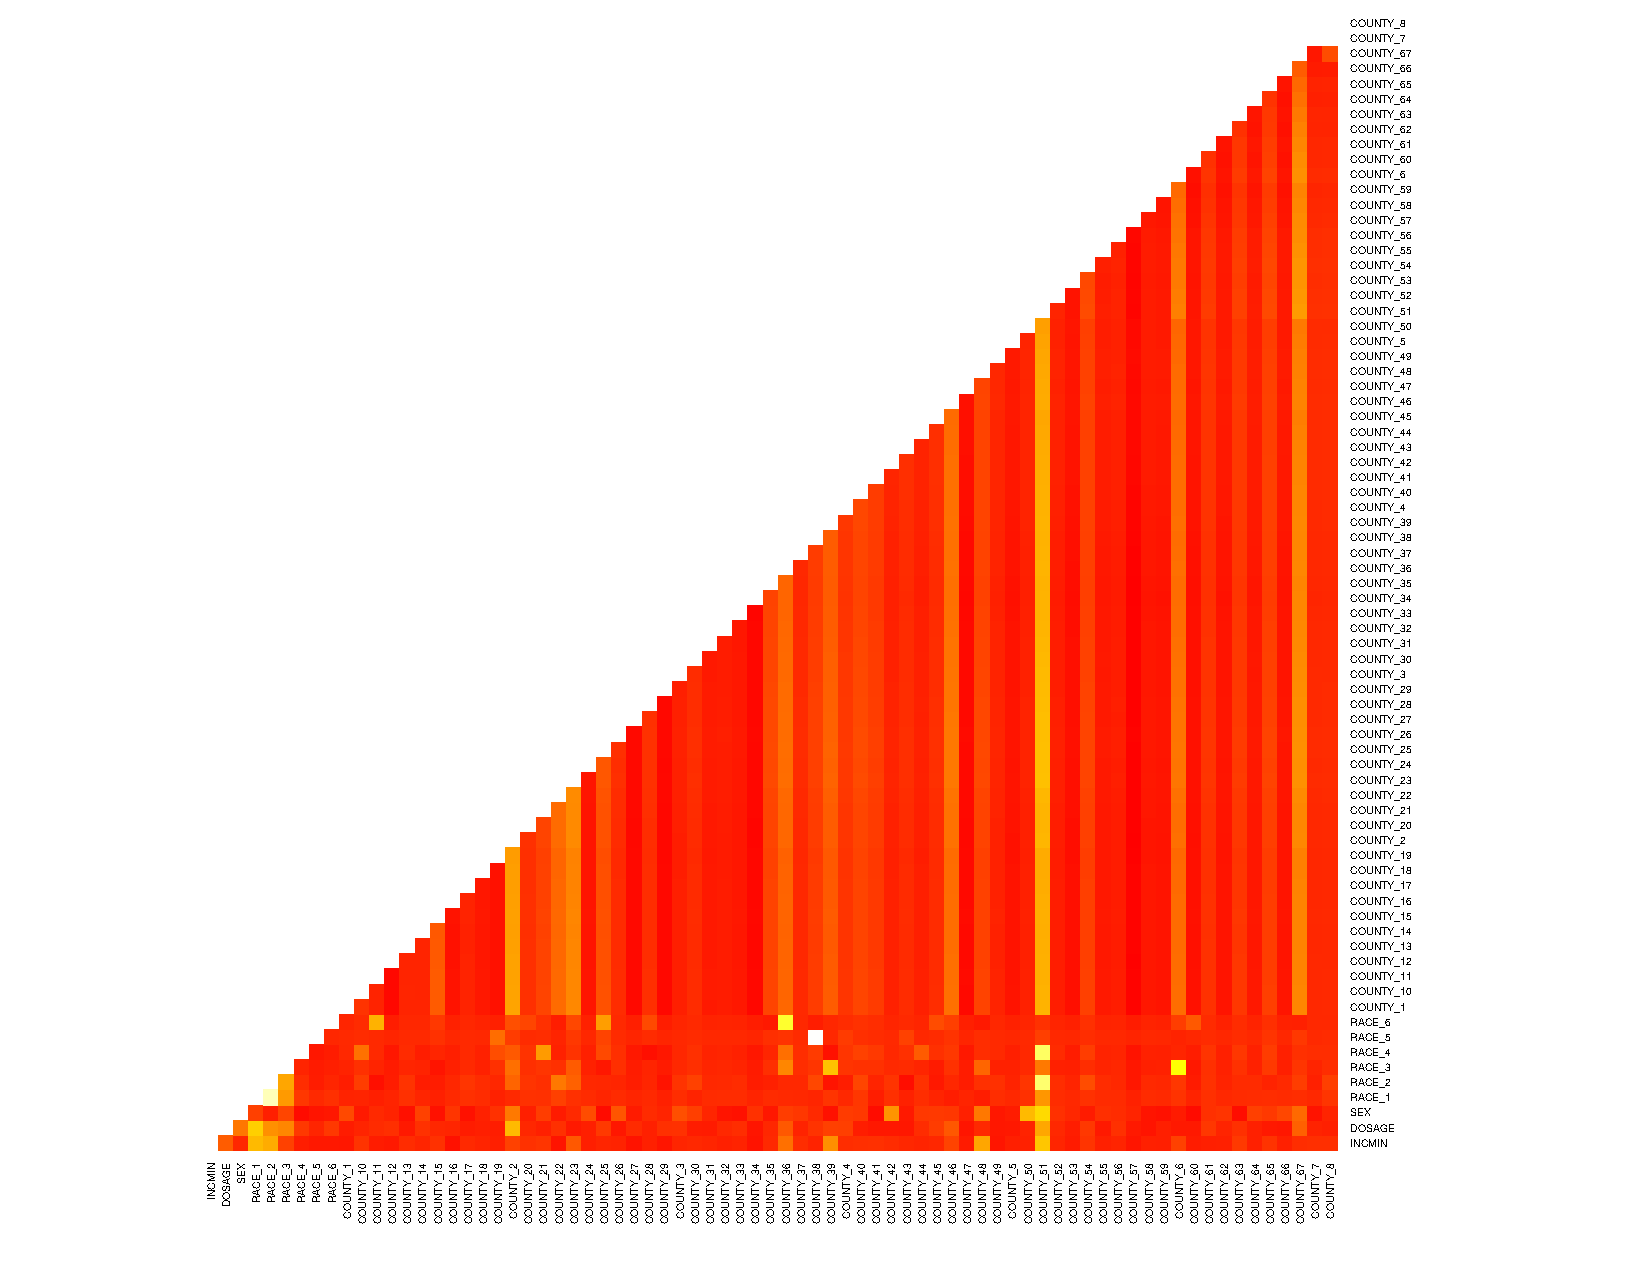
\includegraphics[scale=0.5]{report_figures/demo.pdf}
\subsubsection{CRIME Correlation Heat Map}
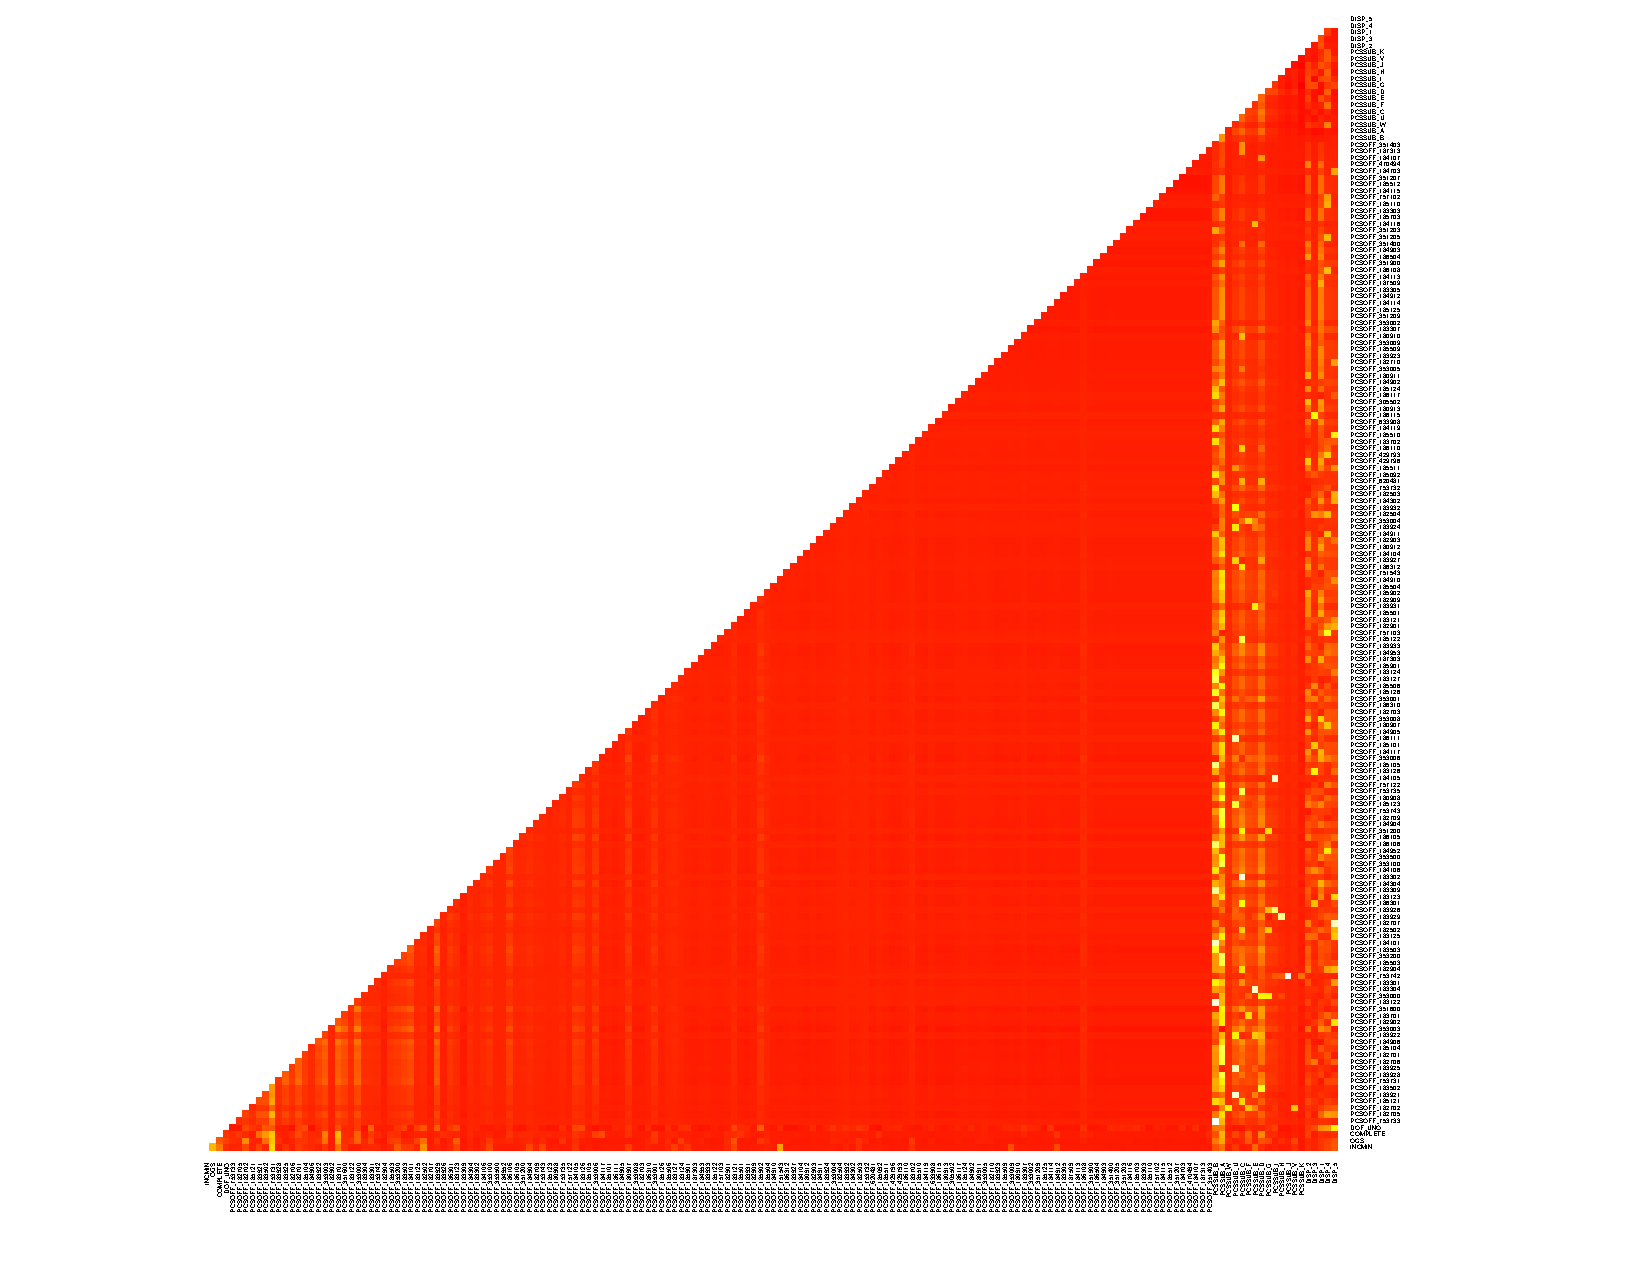
\includegraphics[scale=0.5]{report_figures/crime.pdf}
\subsubsection{ABOUT Correlation Heat Map}
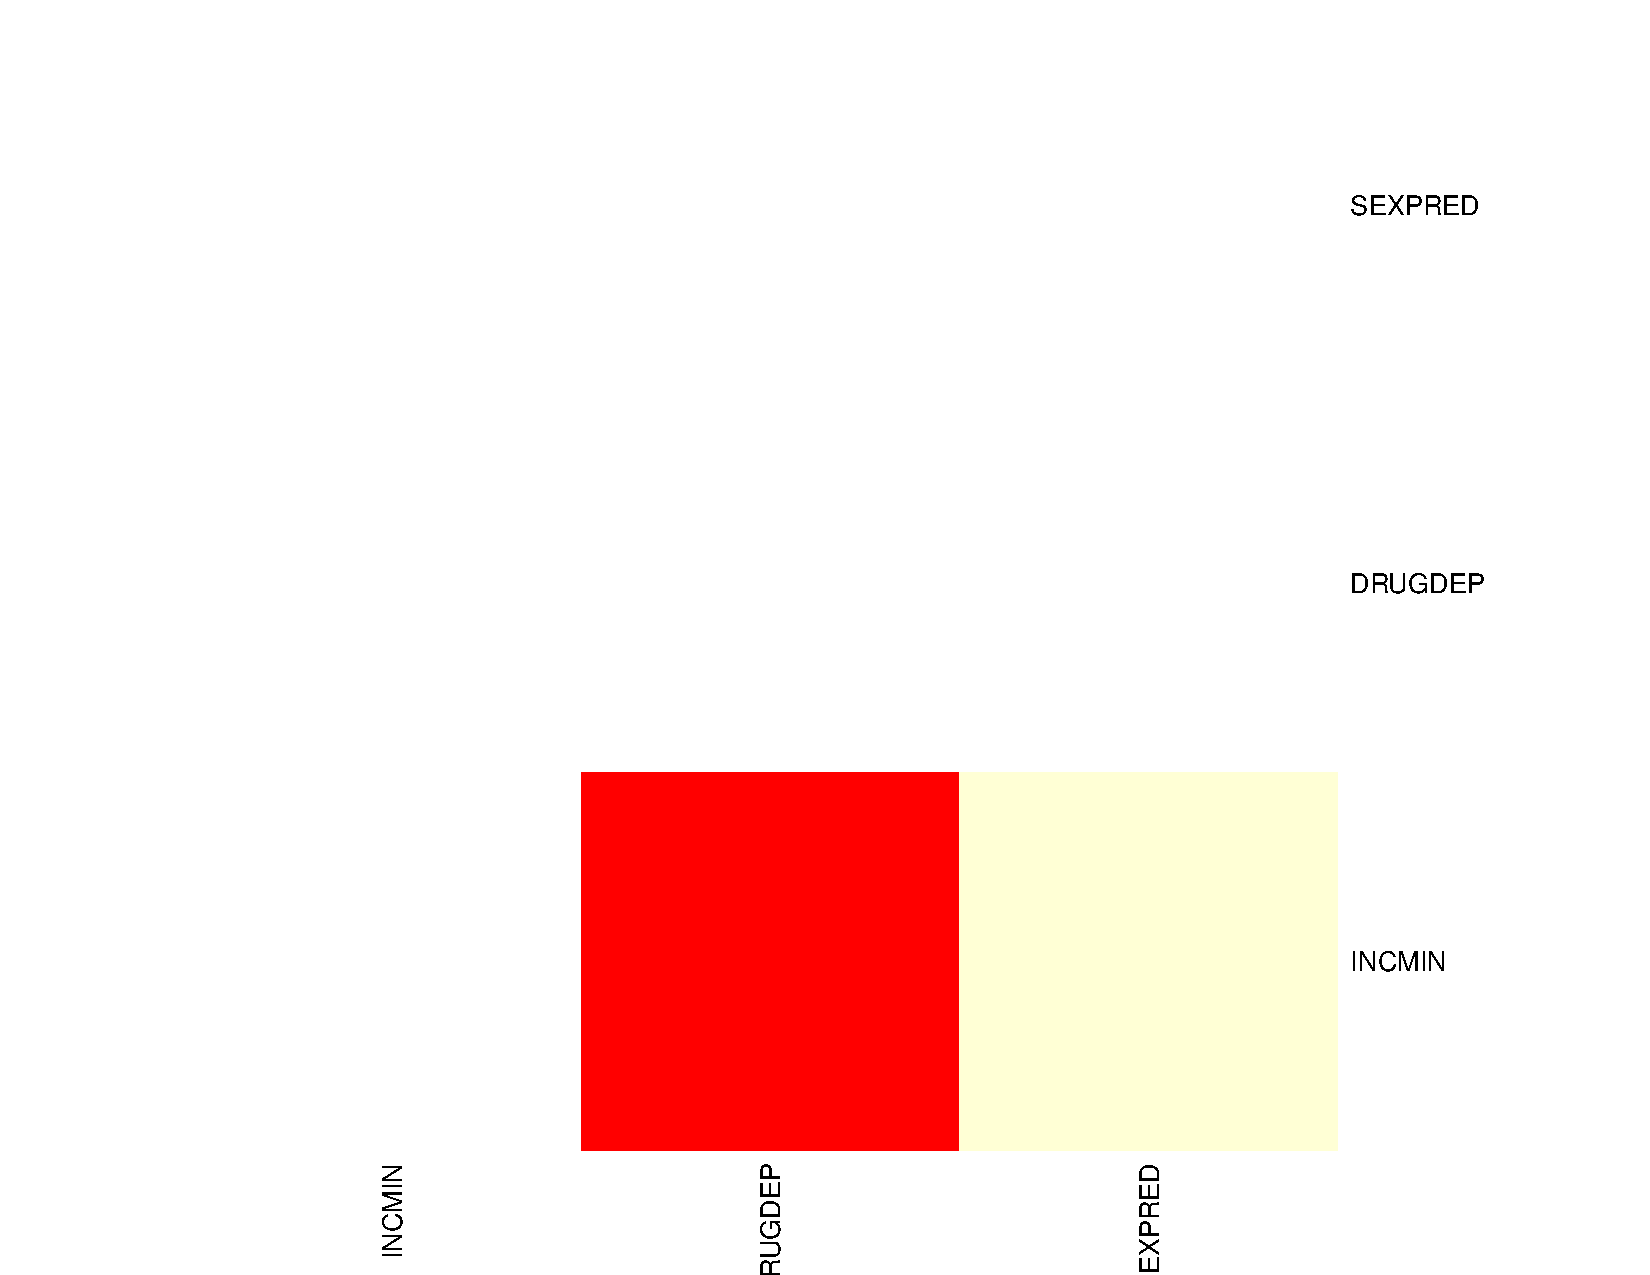
\includegraphics[scale=0.5]{report_figures/about.pdf}
\subsubsection{HIST Correlation Heat Map}
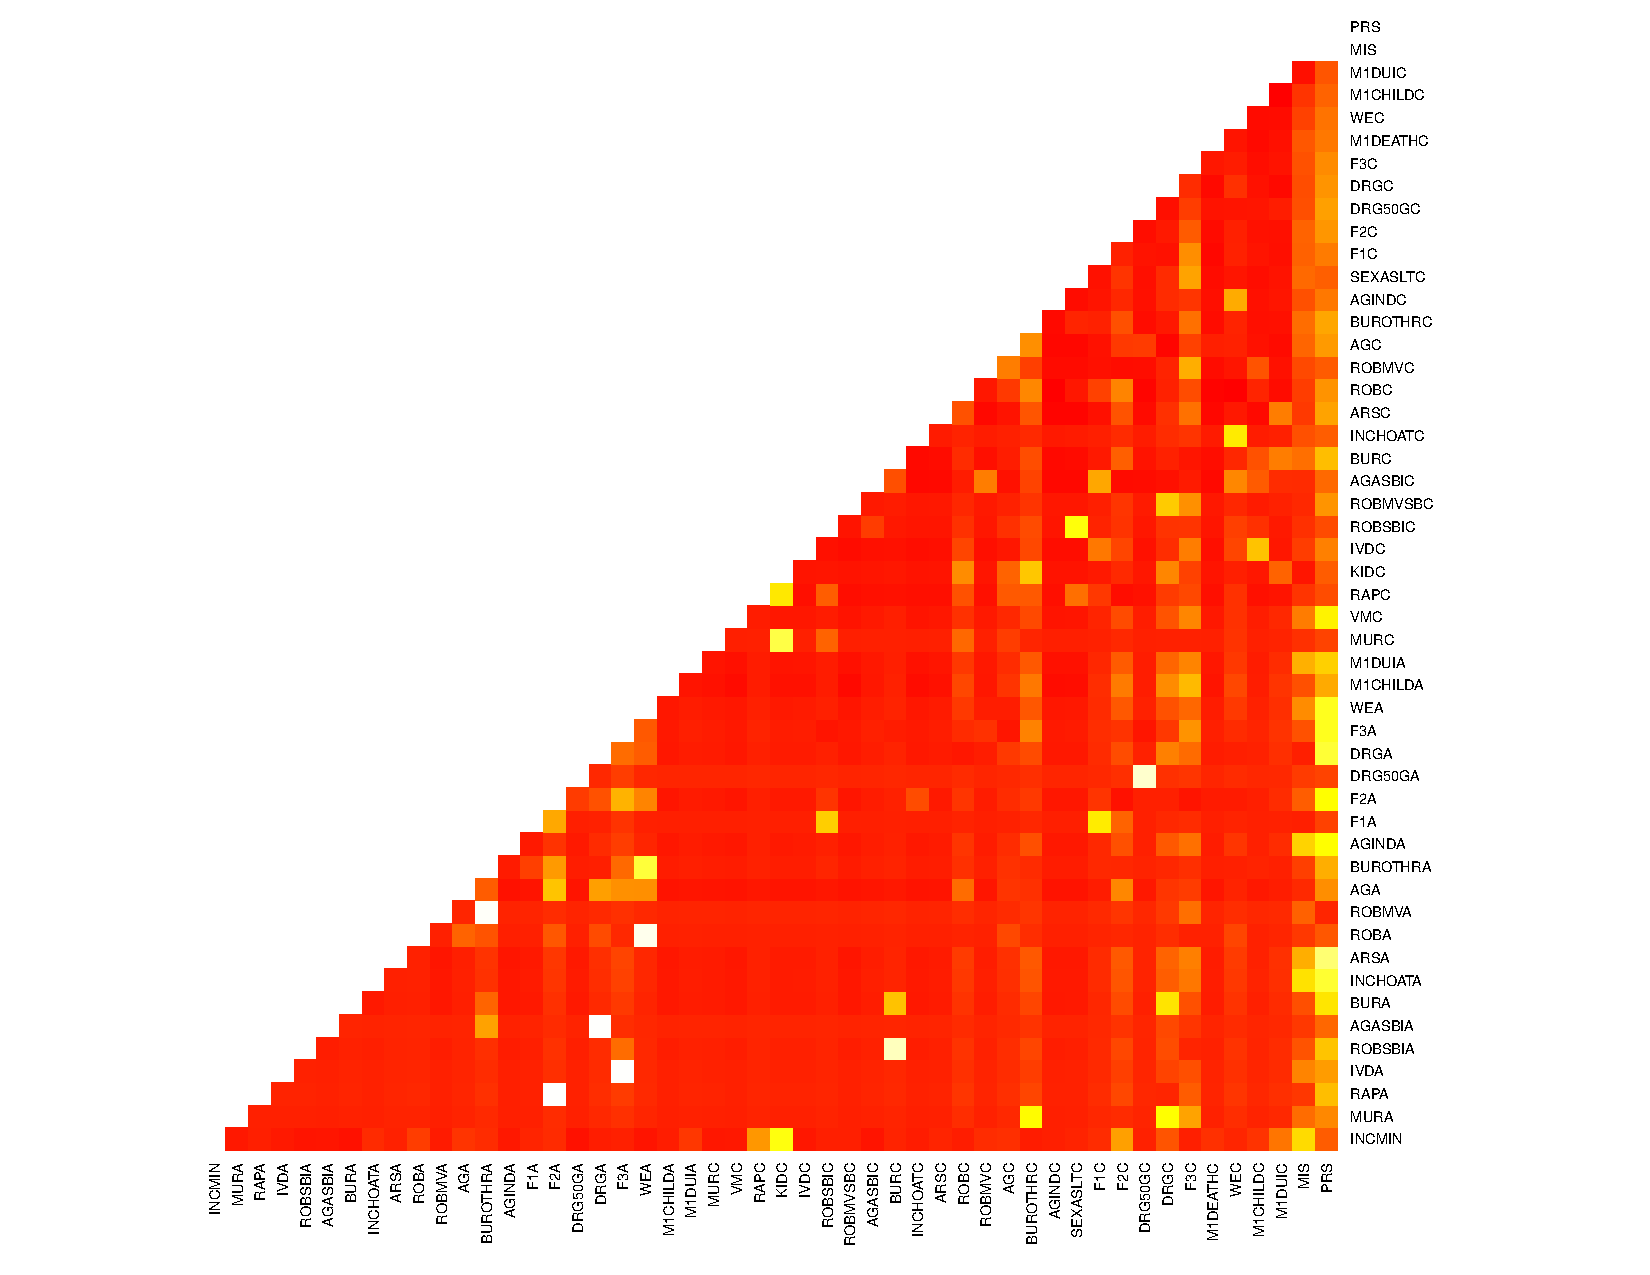
\includegraphics[scale=0.5]{report_figures/hist.pdf}
\subsubsection{ALL Correlation Heat Map}
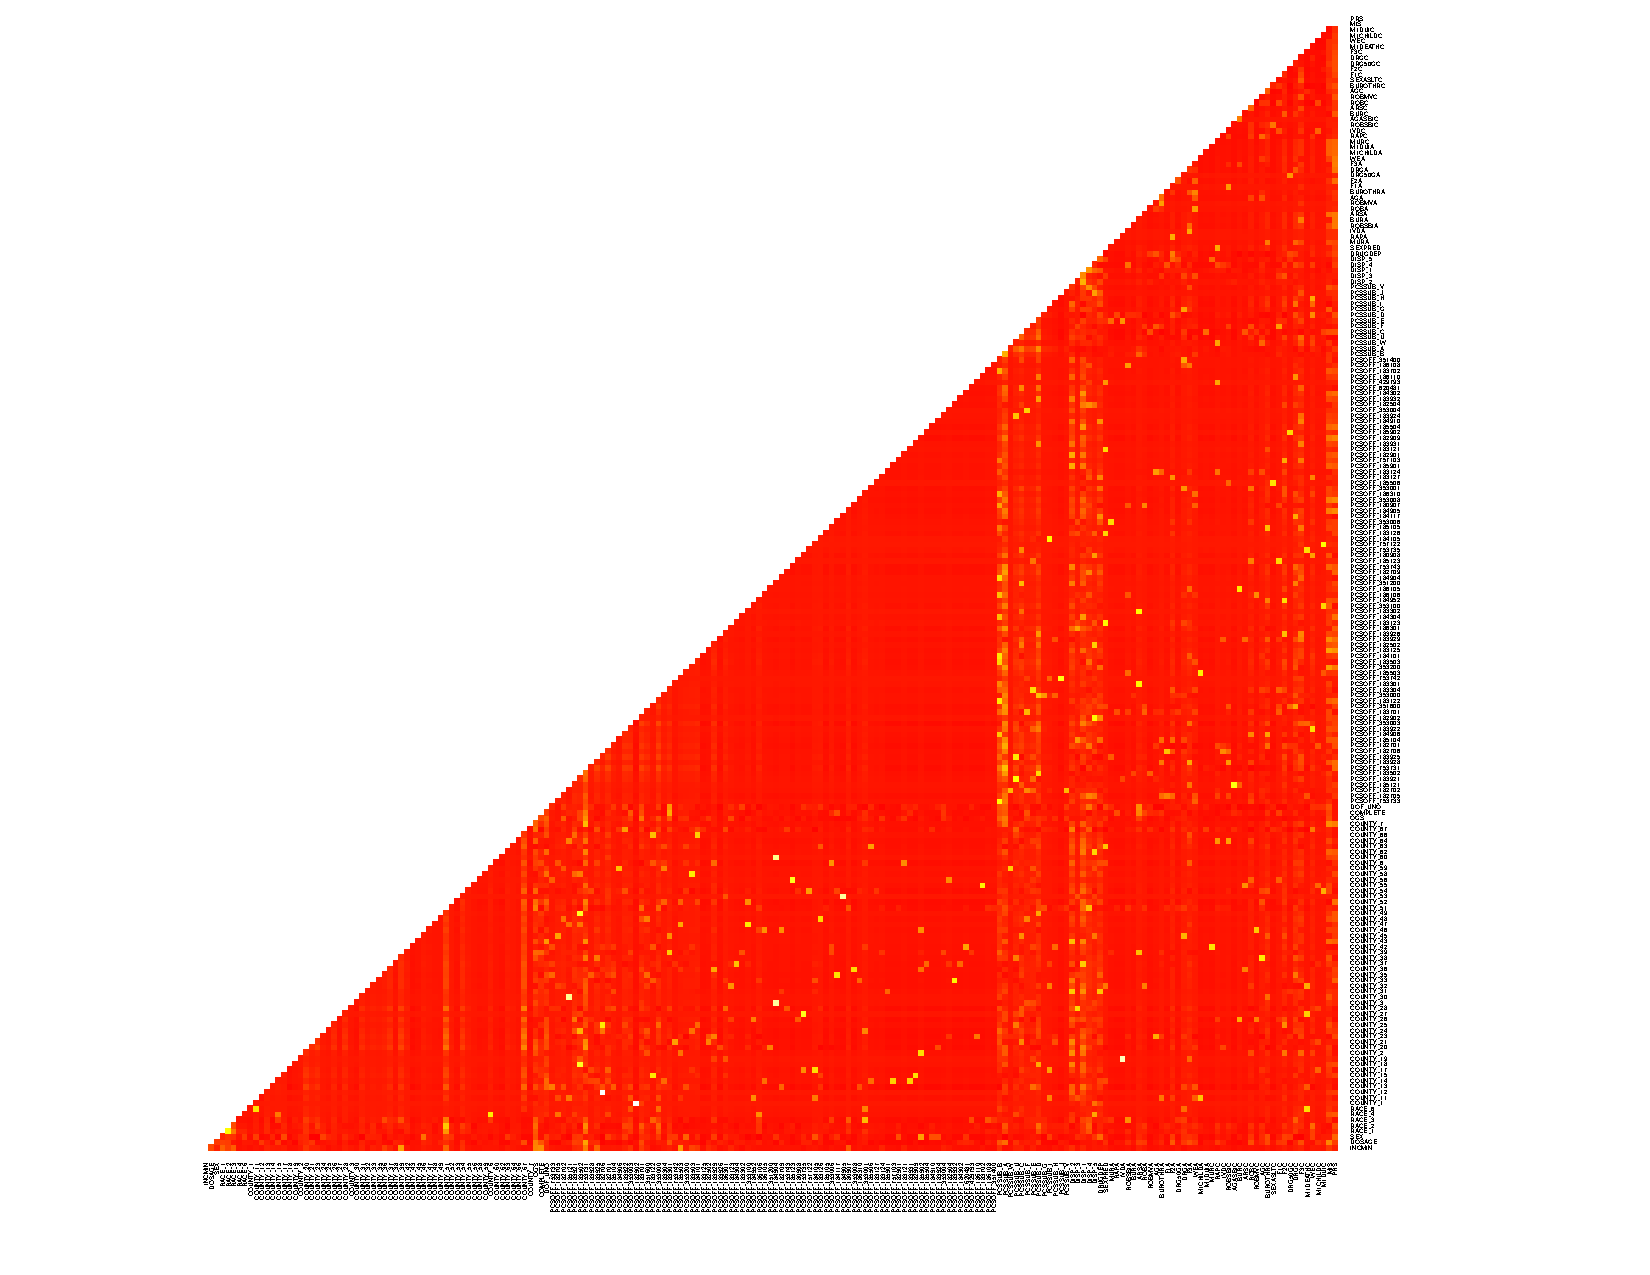
\includegraphics[scale=0.5]{report_figures/all.pdf}

\end{document}